\npchapter{Reference Architecture}
As mentioned in the introduction, this work is written in cooperation with SAP. In fact, the limitations mentioned in the previous chapter are deducted from the limitations the SAP Gardener team struggles with themselves. Subsequently, this chapter introduces the \textit{Open Component Model (OCM)}, SAP Gardener's proposed standard to decouple the compliance scans from the CI/CD pipeline. Based on this knowledge, an overview of the development and deployment landscape of SAP Gardener is given. Finally, the suggested integration of the \emph{Security and Compliance Data Lake}, as a central application for storing and querying software metadata, with the existing standard and landscape is presented. Thereby, this chapter provides a reference architecture on how to overcome the major limitations of the current state of the art approach.

\section{Open Component Model} \label{sec:Open Component Model}
The OCM is a SBOM format created and used by SAP Gardener. It does not fulfill the minimum requirements as defined by the NTIA. But this is due to the fact that the OCM has a different focus than SPDX or CycloneDX. While those two were deliberately designed to be a bill of materials, thoroughly listing the inventory of a software, the OCM was specifically developed to decouple CI from CD and thereby overcome related limitations such as the ones mentioned in the previous chapter.\par 
So, SPDX effectively describes \emph{arbitrary metadata} (e.g. licenses and file type) about logical units of software. SPDX refers to this logical units of software as \emph{Packages}. As described in section \ref{sec:SBOM} "Software Bill of Materials", a \emph{Package} may be anything, ranging from a snippet of code over single file over an artifact to an entire software product version. Thus, SBOMs are \emph{containers for arbitrary software metadata}.\par
Opposed to that, the OCM describes the \emph{delivery relevant information about and the access to artifacts} composing a logical unit of software. OCM refers to this logical units of software as \emph{Components}, or rather \emph{Component Versions}. Thus, \emph{Component Versions} are  \emph{containers for a structured set of delivery relevant artifacts}.\par 
For this reason, SAP Gardener stopped referring to OCM as an SBOM format and instead invented the term \emph{Software Bill of Delivery (SBOD)}.\par
Following is a technical explanation of the OCM deducted from the specification \cite{OCMSpec}, an internal presentation \cite{OCMInternalPresentation} and interviews with responsible developers. Even though this explanation focuses on understanding the rationale behind the design decisions of the proposed standard rather than technical completeness, it may still be hard to grasp at times. This is due to the abstract nature of the OCM. Therefore, emphasis and examples are used where possible. Also, while the textual description really explains the OCM as the abstract model that it is, figure \ref{fig:ComponentDescriptor} below shows an actual \emph{Component Descriptor}, the serialization format of a \emph{Component Version}. This may also support in understanding the abstract concepts.

\subsection{Model Elements}

\noindent\textbf{Component}\\
"A \emph{Component} is an abstract entity describing a dedicated usage context or meaning for provided software. It is technically defined by a \emph{globally unique identifier}"\cite{OCMSpec} (l. 2). With this globally unique identifier, a \emph{Component} acts as a namespace for multiple \emph{Component Versions}. So the \emph{Component} identified by the name \lstinline|github.com/gardener/etcd-druid| contains software versions of a product, a druid, that helps configuring \emph{etcd}, a central key-value store, in Kubernetes clusters' deployed by SAP Gardener.\\

\noindent\textbf{Component Version}\\
As already described, a \emph{Component Version} describes a structured set of concrete \emph{Artifacts}. It is technically defined by the globally unique identifier of the \emph{Component} and a version (ll. 2-3). Thus, a \emph{Component Version} is a instance of a \emph{Component} adhering to the semantic assigned, thus, the usage context or meaning, given by the name. A \emph{Component Version} leverages essentially two mechanisms to describe this structured set of \emph{Artifacts}. 
\begin{enumerate}
\item A \emph{Component Version} may describe the delivery relevant information about and the access to an artifact directly (ll. 9-22, ll. 23-39).
\item A \emph{Component Version} may describe a reference to another \emph{Component Version} to include its described set of artifacts indirectly (ll. 40-56).
\end{enumerate}

\noindent\textbf{Artifacts and Component References}\\
The two model elements enabling those artifact composing mechanisms are \emph{Artifacts} (ll. 9-22, ll. 23-39) and \emph{Component References} (ll. 40-56). Thereby, drawing an analogy to file systems, \emph{Artifacts} and their identities are correspond to files and their names and \emph{Component References} and their identities are analogous to directories and their names.\par
Both those model elements share common sets of attributes \cite{OCMSpec}:\\

\textbf{Identity:} The \emph{Identity} attribute set composes a \emph{Component Version-Local Identity}. Thus, it uniquely identifies the elements in the context of a \emph{Component Version}. The \emph{Identity} at least consists of a \emph{name}.\par 
The \lstinline|name| \emph{(string)}  (l. 10, l. 24, l. 41) is \emph{required} should be chosen to be unique within the \emph{Component Version}. But as it also carries semantic information, the meaning or purpose of the element. So, a \emph{Component Version} may describe a REST application. This REST application may have use a nginx version as HTTP server and a different nginx version as load balancer. In order to have the flexibility to name them both "nginx" the \emph{Identity} has two additional optional attributes, \emph{version} and \emph{extra identity}.\par
The \lstinline|version| \emph{(string)} (l. 16, l. 25, l. 43) is \emph{optional} and describes the version of the respective model elements.\par
The \lstinline|extraIdentity| \emph{(map[string]string)}(l. 17, l. 32, ll. 45-46) is \emph{optional} and allows adding arbitrary identity attributes.\par
As this is a \emph{Component-Version-Local Identity}, \emph{Sources}, \emph{Resources} and \emph{Component References} may be identified by the triple \emph{({Component Name}, {Component Version}, {Local Identity})}.\\

\textbf{Labels:} The \emph{Labels} attribute set is represented by a single \lstinline|labels| \emph{([]any)} attribute. With this, \emph{Labels} allows to attach additional arbitrarily nested metadata to such an element, which is not directly described by the existing model elements. This enables the use of application specific attributes without the need to extend the model for new arising use cases \cite{OCMSpec}. When a \emph{Component Version} is used by a tool to retrieve the artifacts of the respective product version and put them into a scanning tool, a tag within the labels attribute could be used to mark exceptions, e.g. an artifacts within that product version that does never have to be scanned.
\begin{figure}[H]
\begin{minted}[
frame=single,
fontsize=\tiny,
linenos,
numbersep=-10pt,
obeytabs=true
]{YAML}
    component:
      name: github.com/gardener/etcd-druid
      version: v0.15.3
      repositoryContexts:
        - type: ociRegistry
          baseUrl: eu.gcr.io/sap-se-gcr-k8s-private/cnudie/gardener/development
          subPath: null
      provider: internal
      sources:
        - name: github_com_gardener_etcd-druid
          access:
            type: github
            repoUrl: github.com/gardener/etcd-druid
            ref: refs/tags/v0.15.3
            commit: a6112534eb79021fa191edb8efd6512760ae050f
          version: v0.15.3
          extraIdentity: {}
          type: git
          labels:
            - name: cloud.gardener/cicd/source
              value:
                repository-classification: main
      resources:
        - name: etcd-druid
          version: v0.15.3
          type: ociImage
          access:
            type: ociRegistry
            imageReference: >-
              eu.gcr.io/sap-se-gcr-k8s-public/eu_gcr_io/gardener-project/gardener/etcd-druid:v0.15.3-mod1
          digest: null
          extraIdentity: {}
          relation: local
          labels:
            - name: cloud.gardener.cnudie/migration/original_ref
              value: eu.gcr.io/gardener-project/gardener/etcd-druid:v0.15.3
            - name: cloud.gardener.cnudie/sdo/lssd
              value:
                processingRules:
                  - purge_berkeleydb_to_public
          srcRefs: []
      componentReferences:
        - name: etcd
          componentName: github.com/gardener/etcd-custom-image
          version: v3.4.13-bootstrap-8
          digest: null
          extraIdentity:
            imagevector-gardener-cloud+tag: v3.4.13-bootstrap-8
          labels:
            - name: imagevector.gardener.cloud/images
              value:
                images:
                  - name: etcd
                    repository: eu.gcr.io/gardener-project/gardener/etcd
                    resourceId:
                      name: etcd
                    sourceRepository: github.com/gardener/etcd-custom-image
                    tag: v3.4.13-bootstrap-8
      labels: []
    signatures: []
\end{minted}
	\centering
	\caption[Component Descriptor]{Component Descriptor \source{Based on \cite{OCMSpec}}}
	\label{fig:ComponentDescriptor}
\end{figure}

\noindent\textbf{Artifacts}\\
Generally, an \emph{Artifact} is a blob containing some data in some technical format \cite{OCMSpec}. Besides \emph{Identity} and \emph{Labels}, \emph{Artifacts} do have the following further attributes \cite{OCMSpec}:
\begin{itemize}
\item A dedicated globally unique \lstinline|type| (l. 18, l. 26) representing the kind of content and how it can be used.
\item A formal description of the \lstinline|access| (ll. 11-15, ll. 27-30). This description can be used to technically access the content of the artifact in form of a blob with a format defined by the \lstinline|type| of the artifact (l. 18, l. 26) (the \lstinline|type| shown within the access in figure \ref{fig:ComponentDescriptor} specifies the access method and thereby determines the fields of the access specification).
\end{itemize}
The OCM distinguishes two kinds of \emph{Artifacts}, \emph{Sources} and \emph{Resources}.\par
\emph{Sources} (ll. 9-22) describe artifacts that are sources for the delivery relevant artifacts (e.g. source code).\par
\emph{Resources} (ll. 23-41) describe delivery artifacts, intended for deployment into a runtime environment (e.g. executables or OCI Images) or additional content relevant for deployment mechanisms (e.g. helm charts). Thus, these are the artifacts built from \emph{Sources}. The connection may be expressed through the \lstinline|srcRef| attribute which an additional attribute only existing for \emph{Resources} \cite{OCMSpec}.\\

\noindent\textbf{Component References}\\
A \emph{Component Version} may refer to other \emph{Component Versions} by adding a \emph{Component Reference} (ll. 42-58). As already mentioned, through this mechanism, the referring \emph{Component Version} includes the artifact set described by the referred \emph{Component Version}.\par
Important to stress here is, that \emph{Component References} do not only specify the \emph{Identity} of the referenced \emph{Component Version} but do also have the \emph{Component Version-Local Identity}. Thus, the reference itself has an \emph{Identity} within the \emph{Component Version} just like \emph{Artifacts}. Since the name of this \emph{Local Identity} carries the semantic information about the meaning or purpose of the identified piece of software in the context of the \emph{Component Version}, this allows referencing the same \emph{Component Version} twice with different meaning.\par
But since the referenced \emph{Component Version} still has to be specified, the \emph{Component Reference} has an additional attribute, \lstinline|componentName| (l. 44), which, together with \lstinline|version| (l. 45), uniquely identifies the \emph{Component Version} \cite{OCMSpec}.\\

\noindent\textbf{Additional Information}\\
There are some attributes in figure \ref{fig:ComponentDescriptor} are less important, but shall still be mentioned for completeness of the description \cite{OCMSpec}:
\begin{itemize}
\item A \emph{Repository Context} (ll. 4-7) describes the access to an \emph{OCM Repository}. An \emph{OCM Repository} thereby is a repository providing technical access the \emph{Component Version}, or rather the \emph{Component Descriptor}. 
\item The \emph{Provider} (l. 8) specifies the company or organization providing the \emph{Component Version}.
\item A \emph{Component Version} may have \emph{Labels} (l. 59) itself, to attach additional information. 
\item A \emph{Component Version} may be signed by some authority to ensure that it can be trusted. The \emph{signatures} (ll. 60) attribute may contain multiple signatures, where each entry specifies a name for the signature, the digest value for the signature alongside its respective hash- and normalization algorithm and the signature itself. The digest of the \emph{Component Version} thereby includes the digests of the delivery relevant artifacts, thus, the \emph{Resources}, which may be stored alongside their respective descriptions (l. 31).
\end{itemize}

For further or more detailed information about specific elements or the Open Component Model and its ecosystem in general, refer to the official documentation \cite{OCMSpec}.

\subsection{Capabilities of the Open Component Model}
After this abstract description, this brief section revisions the major concepts of and points out the most important capabilities enabled by the \emph{Open Component Model}.\\

\noindent\textbf{Aggregation Mechanism}\\
\emph{Components} and \emph{Component Versions} respectively are an abstract concept, defined in a way that allows to describe the artifact set and its delivery relevant information for arbitrary aggregations ranging from a specific \emph{software product} over \emph{artificial aggregations} like all artifacts used by the SAP Gardener CI/CD team to an entire \emph{application landscape}.\par
So, a \emph{Component Version} named "SAP Gardener CI/CD" could have \emph{Component References} to all \emph{Component Versions} describing a software product used within the SAP Gardener CI/CD team. The \emph{Component Version} hierarchy created through these \emph{Component References} would thereby indirectly specify their complete set of \emph{Artifacts}.\\

\noindent\textbf{Delivery Automation}\\
As each of these \emph{Artifacts} describes the access to the technical artifact in a machine-readable format, a tool may automatically find all the relevant technical artifacts and deploy them into a specific environment or provide them to scanning tools.\par
With that, the Open Component Model enables a \emph{holistic deployment automation} and a \emph{decoupling of compliance scans from the CI/CD pipeline} based on \emph{Component Versions}.\\ 

\noindent\textbf{Technology-Agnostic and Access-Independent Identification Scheme}\\
The OCM introduces a \emph{technology-agnostic identification scheme} based on the component namespace. Thus, an artifact is addressed through its semantic within the \emph{Component} independent of its technology - to be concrete the triple \emph{({Component Name}, {Component Version}, {Local Artifact Identity})}.\par
An \emph{Component Version} might describe a software product. This software product includes an Java library as an \emph{Artifact} with a \emph{Local Artifact Identity}, e.g. "JavaLib". This Java library may be stored in a Maven repository where it is identified by its group id (uniquely identifies a project across all maven projects), artifact id (uniquely identifies a artifact within a project) and version (e.g. org.example:javalib:1.0.0). Furthermore, it is stored in a local artifact repository where it is identified by a digest of its contents.\par
To switch the location where the artifact will be accessed by tools evaluating the \emph{Component Version} describing the artifact, only the \emph{access} has to be exchanged without affecting the identity through which the \emph{Artifact} is addressed.\par 
\emph{By that, the Open Component Model is the link between different storage location (e.g. artifact repositories and source repositories) and tools (e.g. scanning tools).}\par
This is also important in complex development and deployment landscapes as it provides additional flexibility. Due to national restrictions, one might be obligated to deploy artifacts from artifact repositories located in the respective country. Hence, different \emph{Component Repositories} may store \emph{Component Descriptors} for a specific \emph{Component Version} with different \emph{access} properties. Thus, the \emph{access} properties may be exchanged transparently without affecting the deployment automation.\\

While the Open Component Model thereby solves almost all limitations of the current state of the art approach, it does not provide the means to easily answer where Log4j is deployed. \emph{Thus, there is still a need to store this information in a queryable manner alongside other possibly relevant metadata.}

\section{Open Component Model at SAP Gardener} \label{sec:Development and Deployment Landscape at SAP Gardener}
So, SAP Gardener is SAP`s own managed Kubernetes service which enables to easily setup a Kubernetes cluster in the cloud of one of the hyperscalers as well as on premise. In order to provide this service, the team has to maintain a sophisticated development and deployment landscape, which leverages the capabilities of the OCM. Therefore, this section provides a concrete example how to decouple CI from CD using the OCM.\par
A representation of the CI part of the development landscape is illustrated in figure \ref{fig:GardenerCI} below.

\begin{figure}[H]
	\centering
	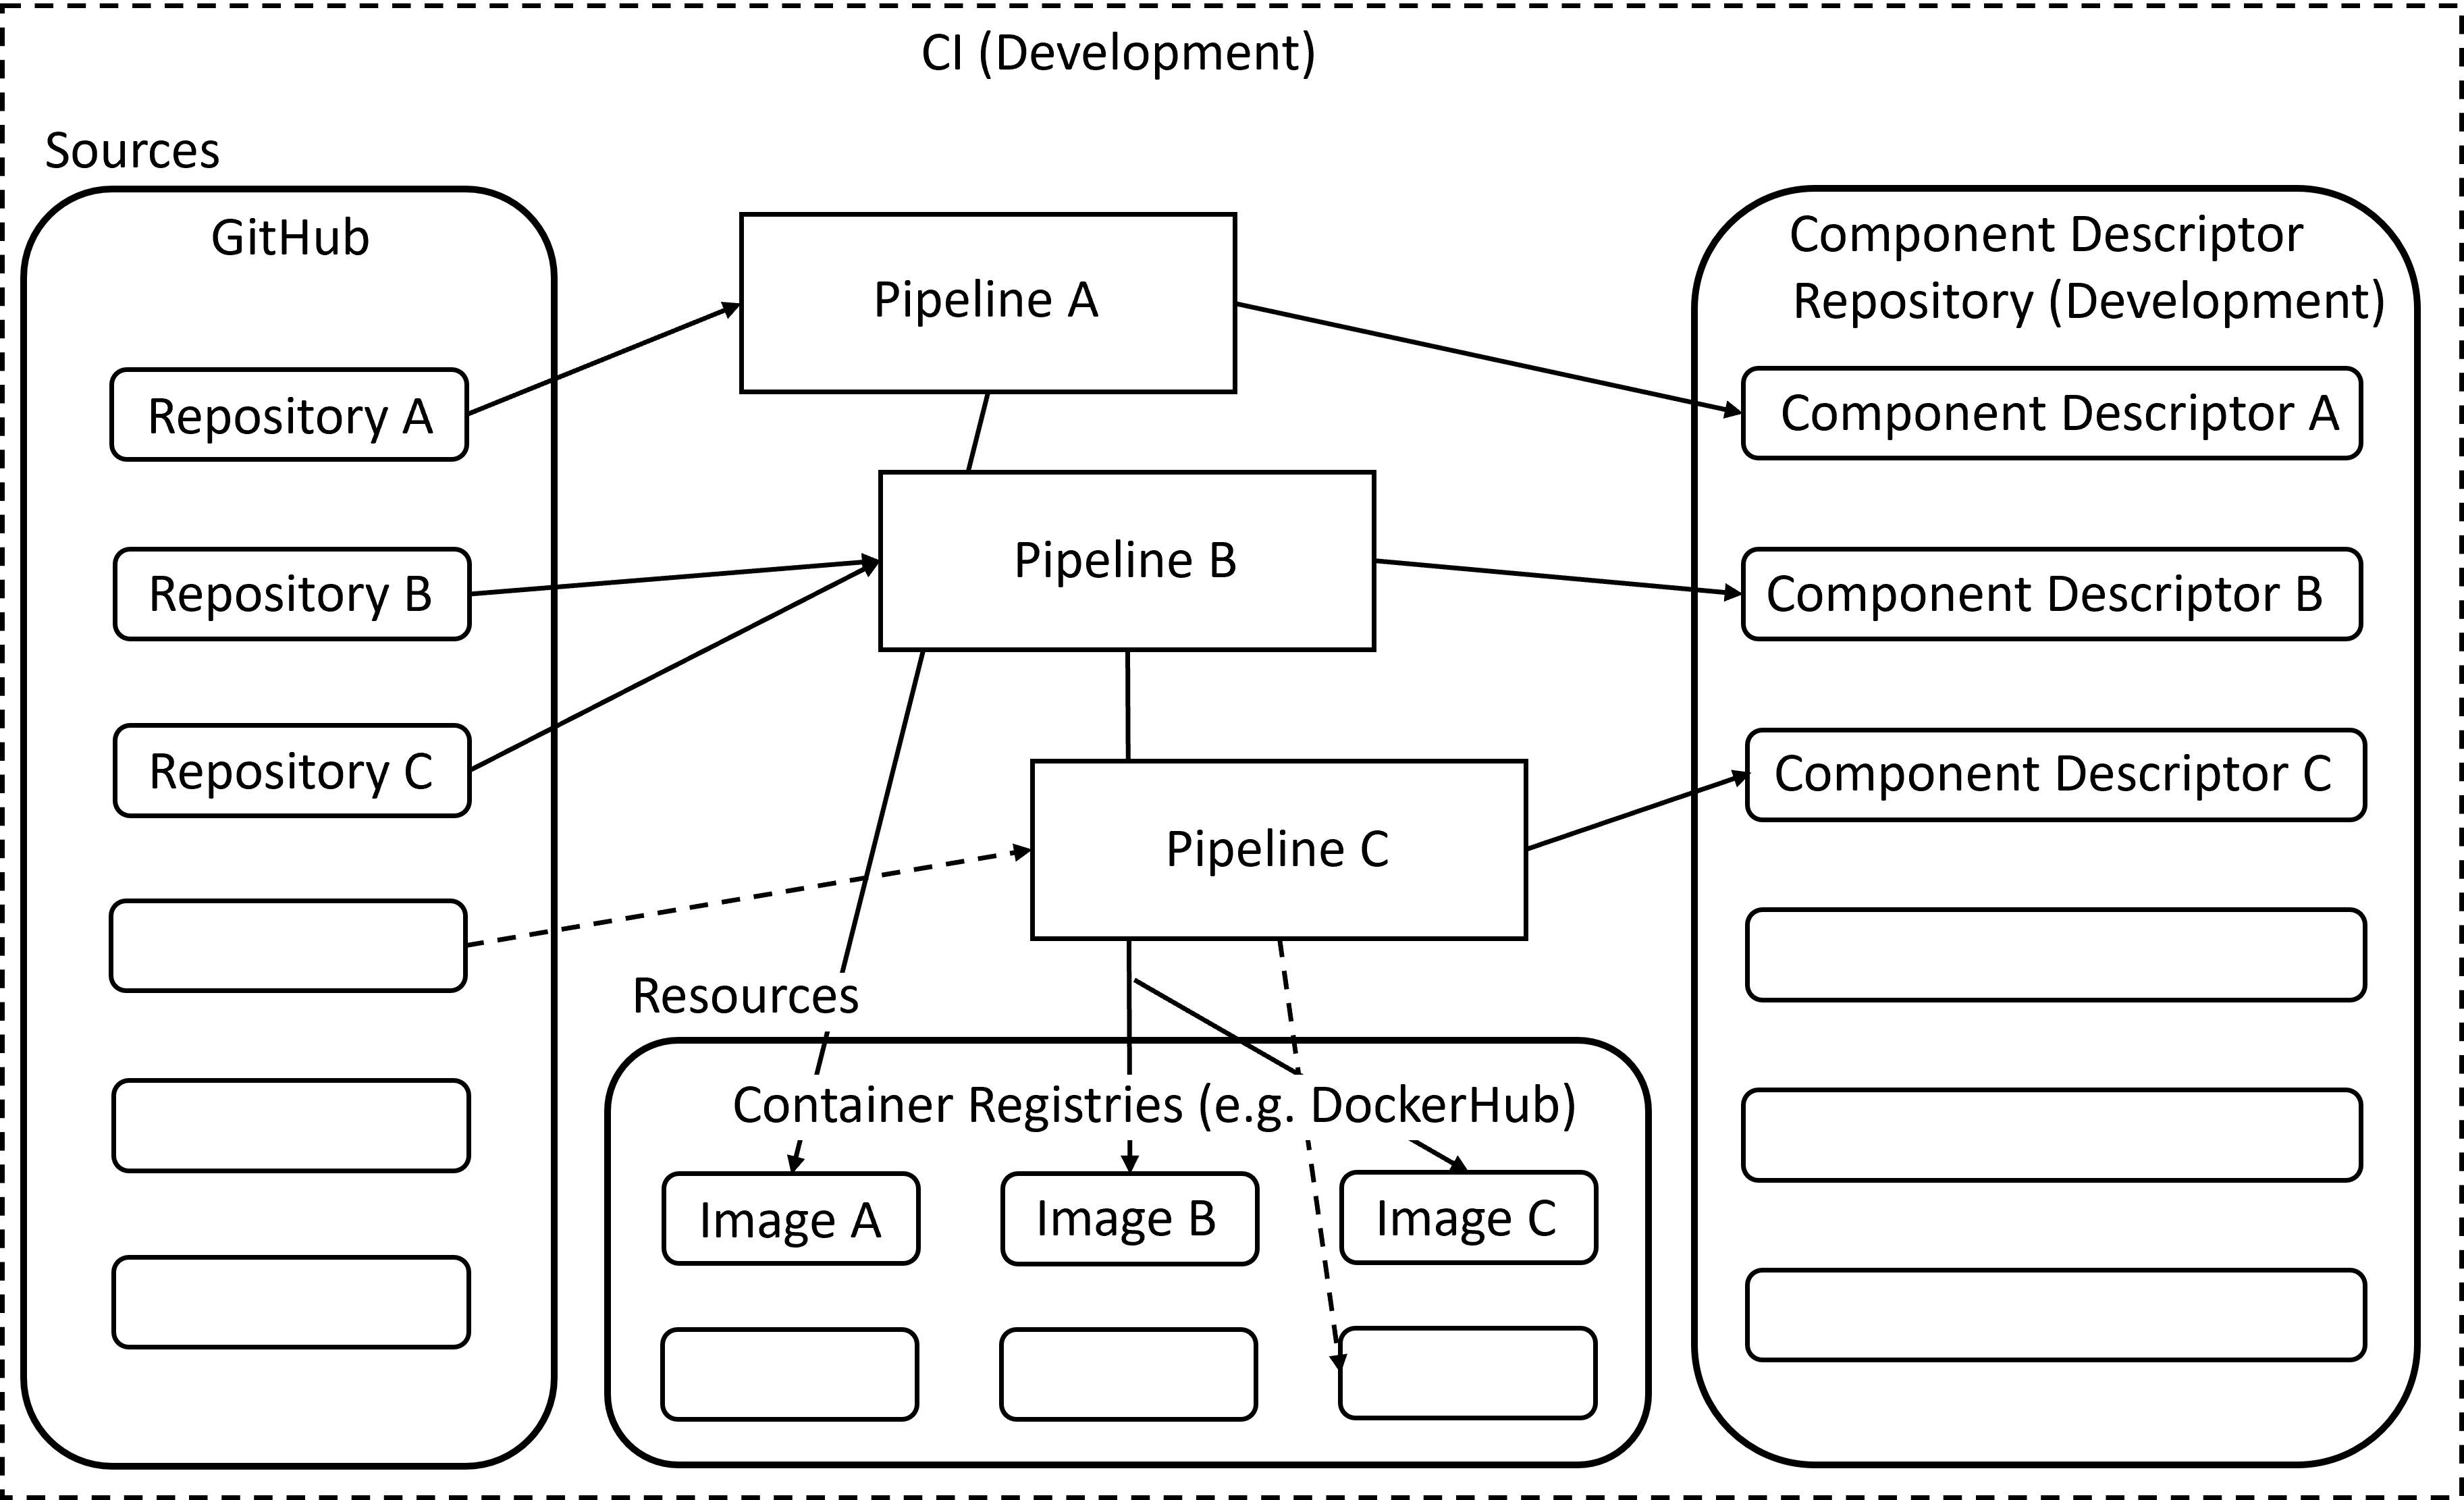
\includegraphics[scale=0.5]{gardener_ci}
	\caption[Gardener CI]{Gardener CI \source{Based on \cite{OCMInternalPresentation}}}
	\label{fig:GardenerCI}
\end{figure}

As shown, there are several sources organized in git repositories hosted on GitHub. Furthermore, there are pipelines for creating the Component Descriptors. These pipelines may build OCI Images from the sources, as indicated by the unbroken lines to Pipeline A and Pipeline B. Instead of actually building, these pipelines may also just use references to existing open source OCI Images and optionally their corresponding sources, as indicated by the dashed arrows. In fact, more than half of the OCI Images powering SAP Gardener are only referenced and not built within the pipeline. Finally, as a result of the pipeline processing, the Component Descriptors are published into the Development's Component Descriptor Repository.\\\\
The next illustration in figure \ref{fig:GardenerCD} is a representation of how this CI system is connected to the CD system.

\begin{figure}[H]
	\centering
	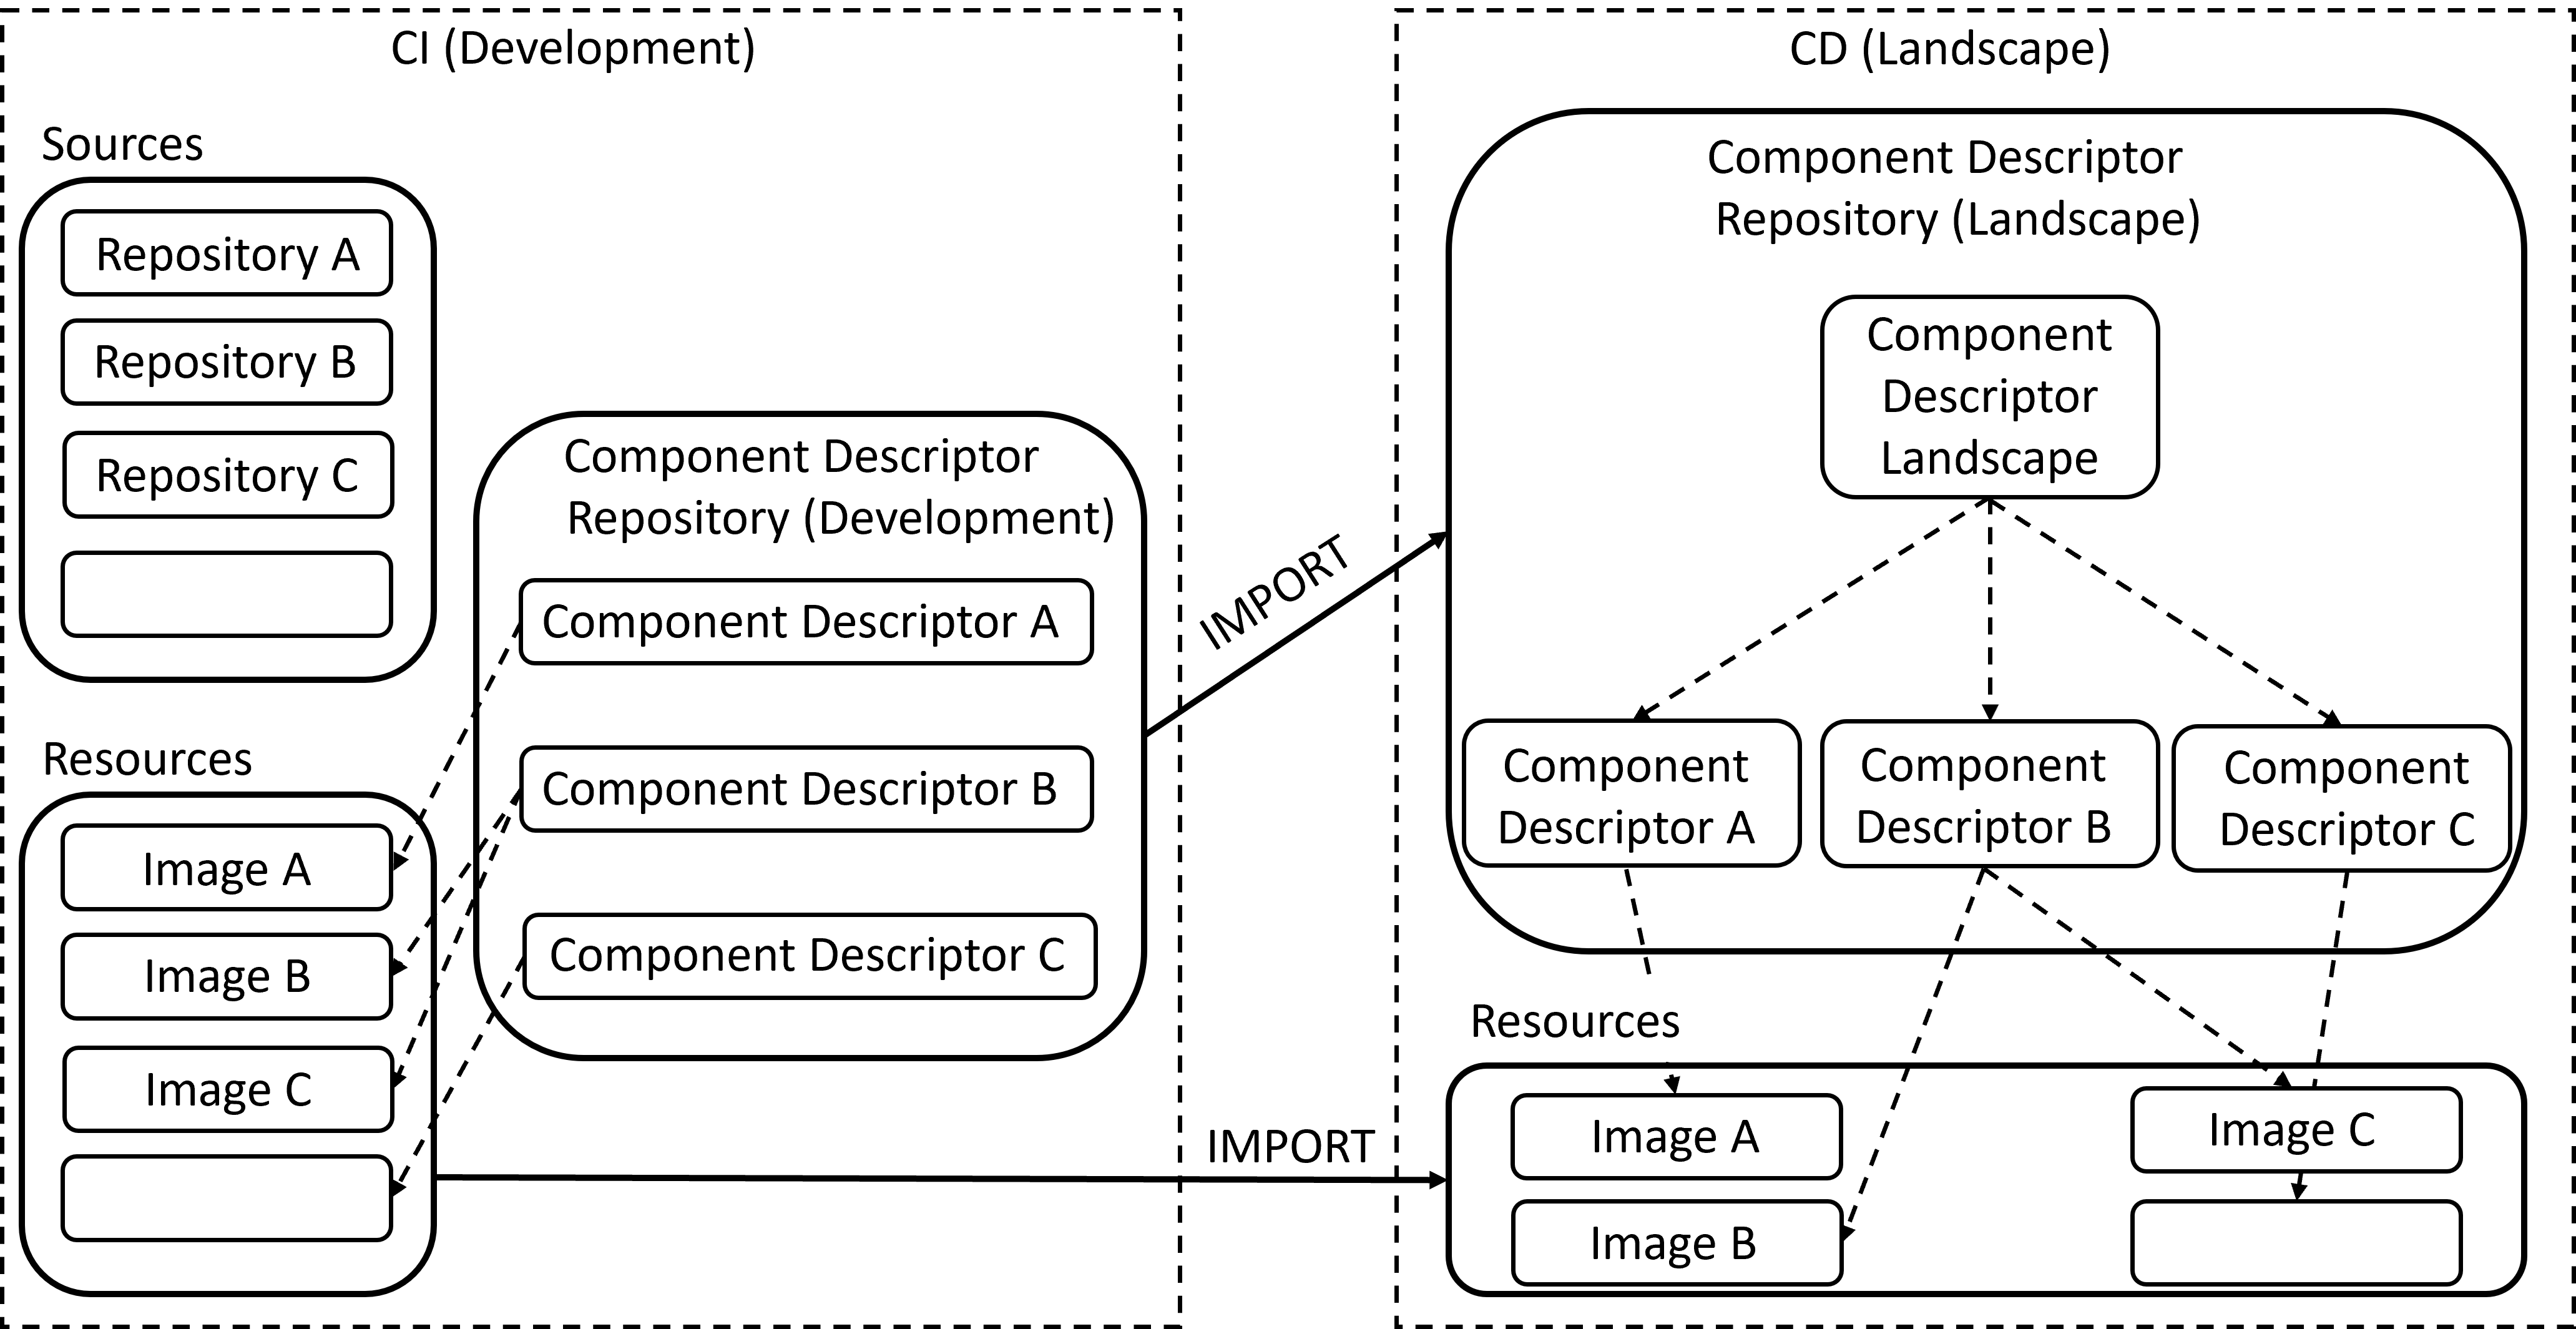
\includegraphics[scale=0.45]{gardener_cd}
	\caption[Gardener CD]{Gardener CD \source{Based on \cite{OCMInternalPresentation}}}
	\label{fig:GardenerCD}
\end{figure}
 
The left side, CI (Development) is a condensed view of figure \ref{fig:GardenerCI}. The dashed arrows represent references. Since the references to the sources stay exactly the same, these dashed arrows are omitted to avoid even more clutter.\par 
So, whenever a new Component Version is released through the CI system, the CD system discovers and imports the corresponding Component Descriptors together with the referenced resources into Component Descriptor and Artifact Repositories of the respective landscape. Thereby, while essentially still referencing the same OCI Images, the access property of these Resource References of the replicated Component Descriptors is adjusted to the OCI Images in the landscapes Artifact Repository. Also, as shown in the illustration, in SAP Gardener, an additional Component Descriptor for a Landscape Component gets automatically created. It references all the Component Versions in a given snapshot of SAP Gardener. Every time a new Component Version is released in the CI system, a new Component Version of this Landscape Component is created.\par 

\begin{figure}[H]
	\centering
	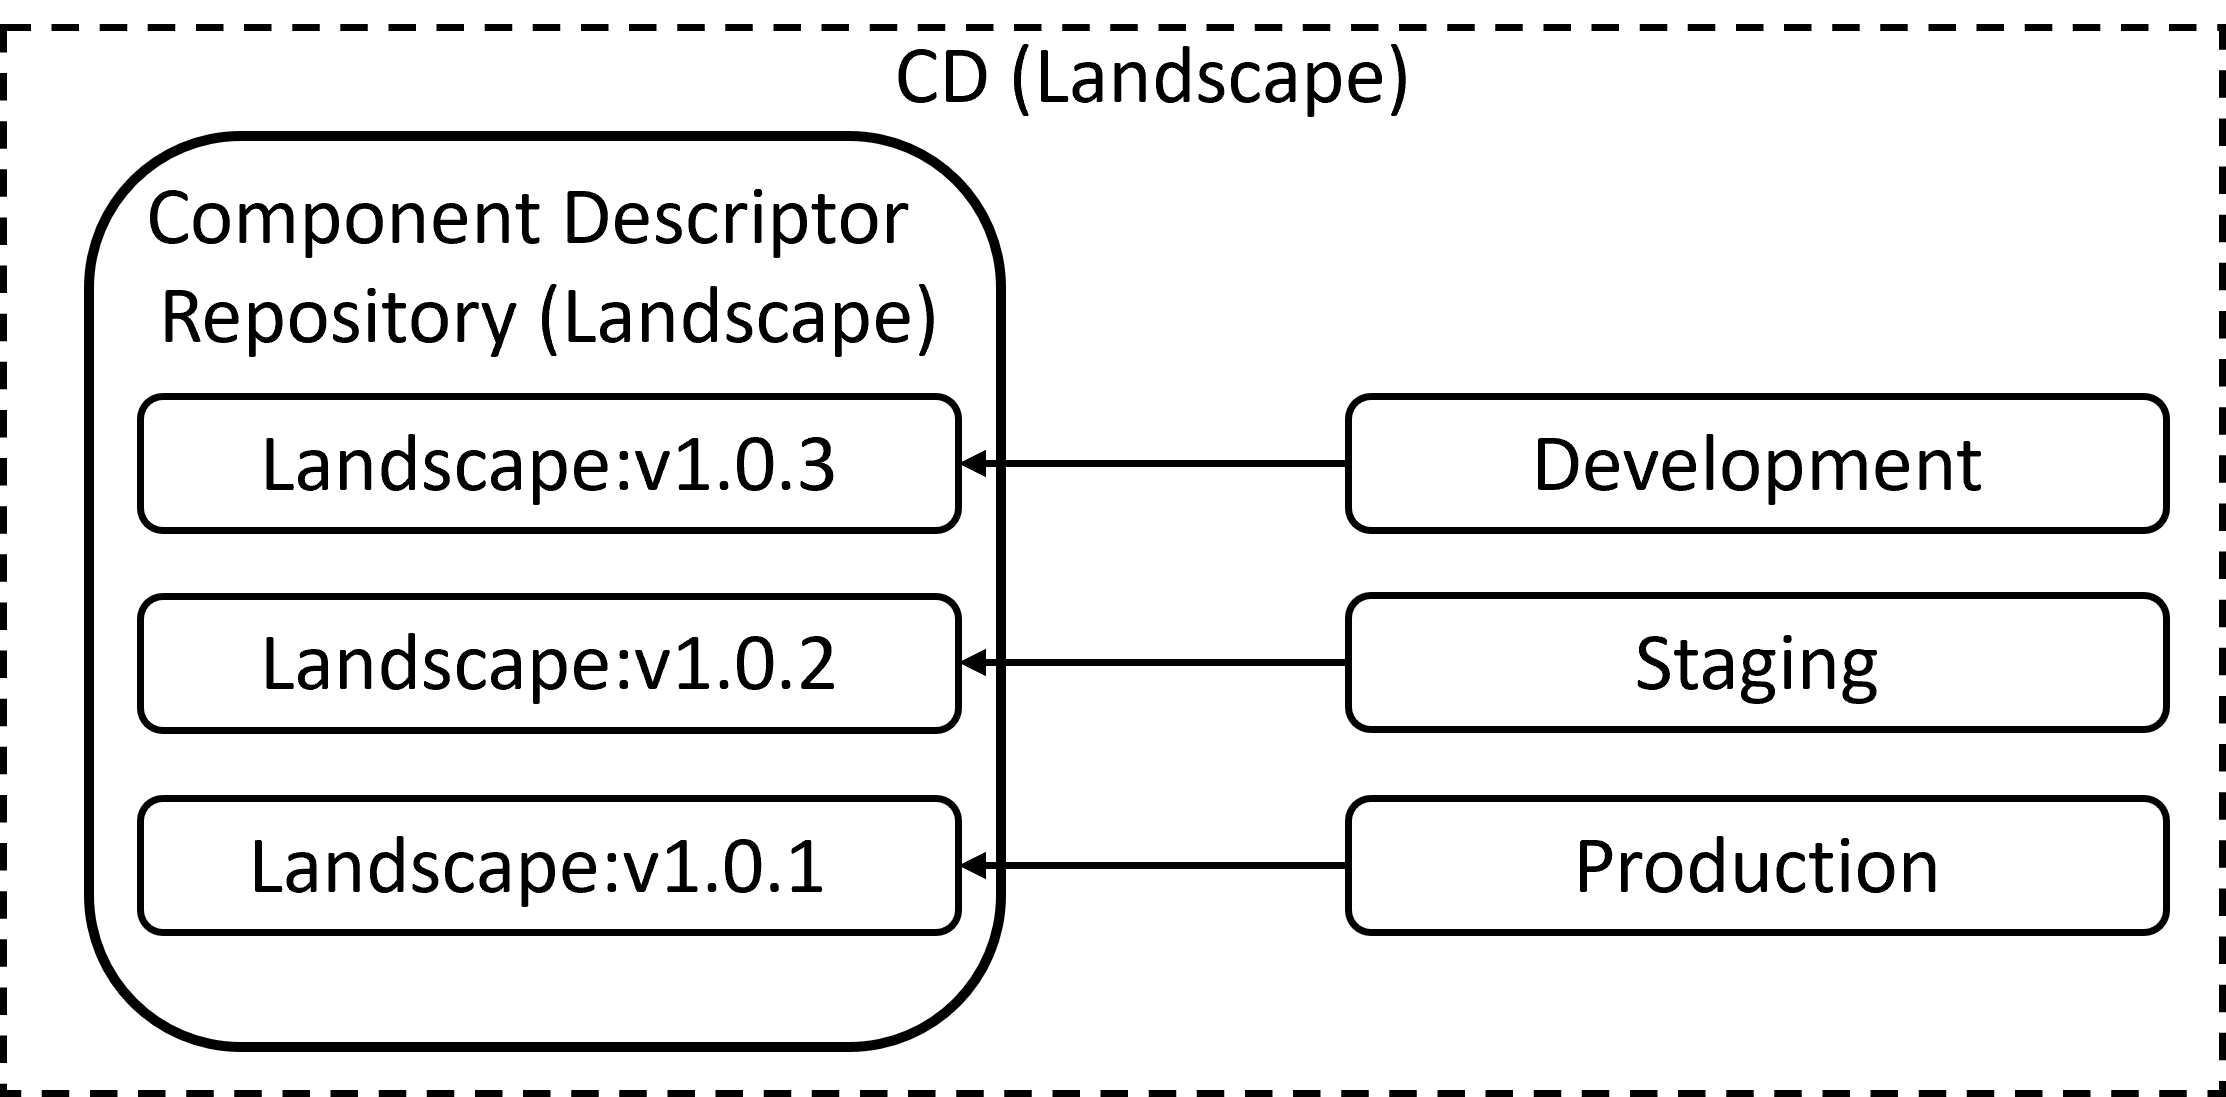
\includegraphics[scale=0.5]{gardener_deployments}
	\caption[Gardener Deployments]{Gardener Deployments \source{Based on \cite{OCMInternalPresentation}}}
	\label{fig:GardenerDeployments}
\end{figure}

Finally, figure \ref{fig:GardenerDeployments} indicates how this setup and particularly the Landscape Component is leveraged to actually deploy an instance of the SAP Gardener. Therefore, the Component References of a Landscape Component Version are traversed and the referenced resources deployed. As usual, the Production deployment is based on an older Landscape Component Version than the Development deployment. 


\section{Integration of the Security and Compliance Data Lake into the SAP Gardener Landscape} \label{sec:Integration of the Security and Compliance Data Lake into the SAP Gardener Landscape}
As already indicated in the previous chapters, although the \emph{Security and Compliance Data Lake} is an application for storing all kinds of metadata, the initial primary use case is storing the data resulting from compliance scans, thus dependencies, vulnerabilities and licenses. Below figure \ref{fig:DataLakeIntegration} shows the architecture designed for the integration into this complex environment of SAP Gardener.\par 
The \emph{Data Collection Service} is the central component of this architecture. Its job is to fetch all the information that shall be stored in the \emph{Data Lake}. In practice, this would be done based on policies, requiring to do such a fetching once a day or based on some kind of event. In order to actually fetch the information, the Data Collection Service sends a request to the \emph{Access Service} (1).\par
The Access Service is a transparency layer already built into the \emph{Component Repositories} as part of the OCM. Thus, if the Data Collection Service requests a set of Component Versions and their referenced Artifacts, the Access Service first fetches the corresponding Component Descriptors from the Component Repository (2). After receiving this information, the Access Service evaluates the access property in the referenced Sources and Resources and sends respective requests to the \emph{Source} and \emph{Resource Repositories} to fetch the Artifacts (3). Finally, the Access Service may return all the requested information to the Data Collection Service.\par

\begin{figure}[H]
	\centering
	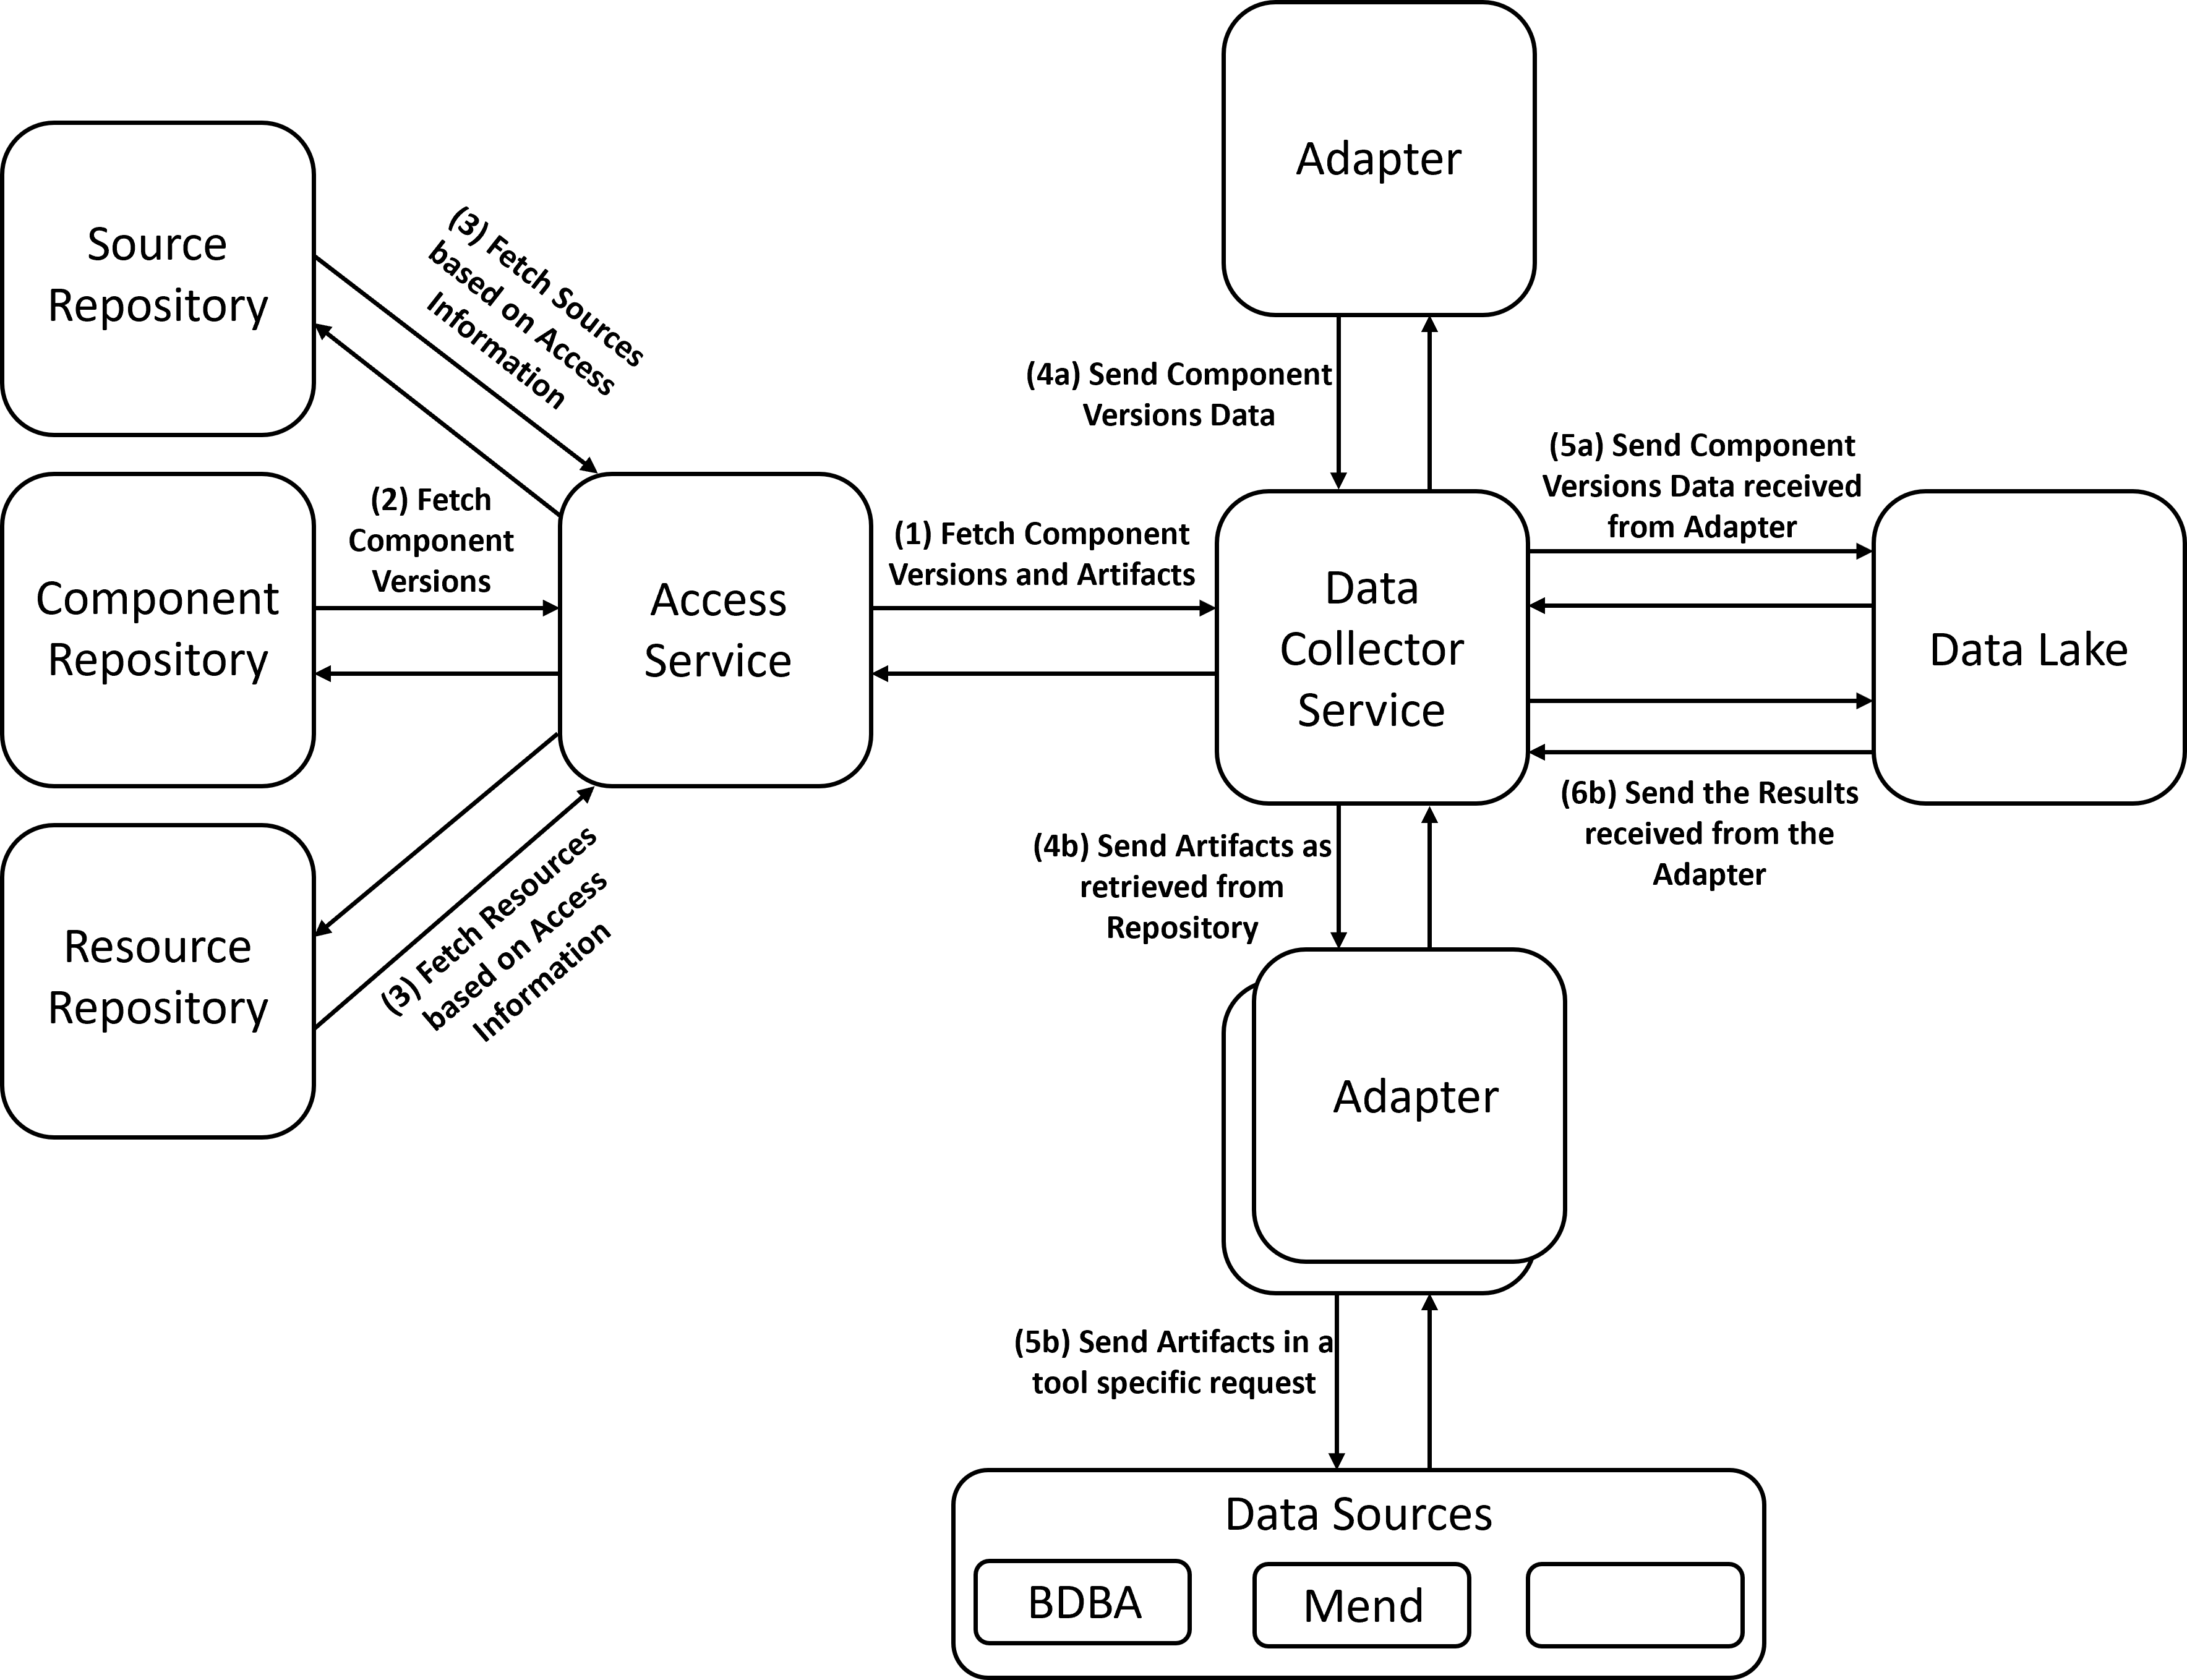
\includegraphics[scale=0.5]{datalake_integration}
	\caption[Data Lake Integration]{Data Lake Integration \source{Own Representation}}
	\label{fig:DataLakeIntegration}
\end{figure}

As shown in the figure, based on this information, there are two requests flows that may be triggered by the Data Collection Service (4a) and (4b). The request flow illustrated above the Data Collection Service (4a) sends the Component Versions data, so the Component Descriptors, to an \emph{Adapter} which adjusts and returns this data in the format required for the consumption by the Data Lake.\par 
The request flow below the Data Collection Service (4b) distributes the Artifacts to a set of Adapters. Here, the Adapters initially wrap the Artifacts into the format required by a specific Data Source. In this case, there would be an Adapter for each compliance scanner. Upon receipt of the scan results, these Adapters also adjust the data to the format required for consumption by the Data Lake, before returning it to the Data Collection Service.\par 
Finally, the Data Collection Service may send all the information, thus, the information acquired from the Component Versions about Components, Resources, Sources and their relationships (5a) as well as the information from the scanning tools about dependencies, vulnerabilities and licenses within these Artifacts (6b) to the Data Lake.\par
There were no communication protocols mentioned so far. This is due to the facts, that it does not really matter on the conceptual level and that the final implementation of this integration architecture is out of the scope of this work. But in practice, the communication between Data Collection Service and Access Service, between Adapters and Data Sources and between Data Collection Service and Data Lake will be over HTTP. The Adapters however will most likely not be implemented as discrete services but as components within Data Collection Service and therefore communicate over shared memory. Since it is very likely that additional Data Sources shall be added later on, the important part on the conceptual level is to still logically separate the components. Thus, there should be well defined interfaces between the Adapters and the Data Collection Service.

TODO: nicht Component Descriptor im Repository sondern Component Versions
TODO: Arbeit beinhaltet auch einen einfach PoC davon



